\section{Méthodes d'apprentissage avec maître distant}
Nous allons observer différentes architectures intéressantes dans le cas de génération de commandes.
Le mot \enum{architecture} utilisé ici ne désigne pas l'architecture d'un réseau de neurones mais l'architecture d'une méthode utilisant des réseaux de neurones dont la convention graphique est montré dans la Figure \ref{legendearchi}.
\begin{figure}
 \centering
 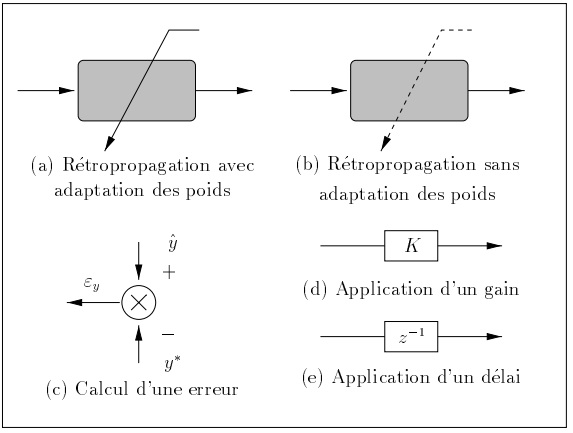
\includegraphics[scale=0.6]{../figures/applegende.jpg}
 \caption{Conventions graphiques pour la descriptions de l'architecture d'une méthode utilisant des RNA. \textbf{Source}: Gauthier\cite{Gauthier}}
 \label{legendearchi}
\end{figure}

\subsection{Le problème}
Dans cette section, nous allons voir différentes méthodes pour entrainer un réseau de neurones pour générer des commandes.
Ces méthodes visent à contourner le \emph{problème de l'apprentissage avec maître distant}.
Dans l'apprentissage supervisé, un \emph{maître} est ce qui permet de fournir une erreur entre la sortie d'un réseau de neurones et la sortie attendue.
Et effectivement dans notre cas, nous n'avons rien qui puisse nous permettre de définir les commandes idéales à éxécuter pour passer d'un certain état à l'autre.
Par contre nous pouvons avoir un maître qui compare l'état résultant de l'éxécution d'une commande à l'état cible.

Dans les architectures qui suivront, le Système désigne l'application, dans la réalité, de la commande entrée et le passage à l'état suivant.

\subsection{Reproduction d'un contrôleur}
\begin{figure}
 \centering
 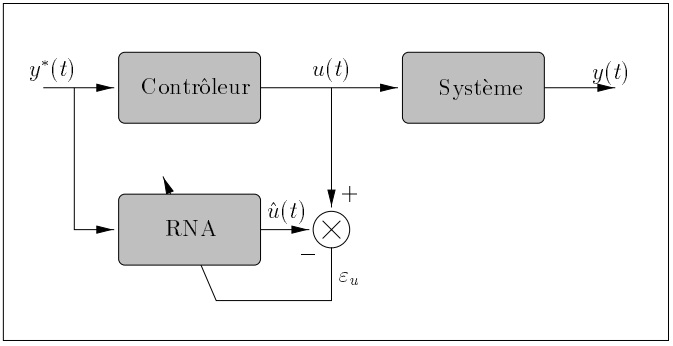
\includegraphics[scale=0.5]{../figures/appsimple.jpg}
 \caption{Apprentissage par reproduction d'un contrôleur. \textbf{Source}: Gauthier\cite{Gauthier}}
 \label{appcontroleur}
\end{figure}
Dans cette méthode d'apprentissage, le \rna apprend à reproduire les commandes d'un contrôleur existant (\textbf{Figure \ref{appcontroleur}}).
Cette méthode a été utilisé pour commander le volant d'une voiture pour suivre des virages où le controlleur est un humain.\cite{Pomerleau}

\subsection{Apprentissage spécialisé}\label{sec:appspecial}
\begin{figure}
 \centering
 
\includegraphics[scale=0.5]{../figures/invalid.png}
 \caption{Apprentissage spécialisé. \textbf{Source}: Gauthier\cite{Gauthier}}
 \label{appspecialise}
\end{figure}
Ici on applique l'algorithme de rétropropagation depuis l'erreur donnée par le maître distant en traversant le système (\textbf{Figure \ref{appspecialise}}).
Nous avons vu que, dans le cas d'un \mlp, section \ref{sec:appmlp}, l'apprentissage est l'application de la formule \[\Delta W_{ij} = -\eta\partiel{Q}{W_{ij}} = \partiel{Q}{\phi_i} \partiel{\phi_i}{v_i} \partiel{v_i}{W_{ij}}\]
En reprenant la notation de la Figure \ref{appspecialise}, \[\Delta W_{ij} = -\eta\partiel{\varepsilon_y}{W_{ij}} = \partiel{\varepsilon_y}{\hat{u}} \partiel{\hat{u}}{v_i} \partiel{v_i}{W_{ij}}\]
Où $v_i$ est la somme pondérée des entrées du neurones $i$.
Or $\partiel{\varepsilon_y}{\hat{u}} = \partiel{\varepsilon_y}{y}\partiel{y}{\hat{u}}$. Et donc la formule devient
\[\Delta W_{ij} = \partiel{\varepsilon_y}{y} \partiel{y}{\hat{u}} \partiel{\hat{u}}{v_i} \partiel{v_i}{W_{ij}}\]
Et connaître le facteur $\partiel{y}{\hat{u}}$ est la difficulté de cette méthode:
Il faut pouvoir modèliser le système par une fonction $y(\hat{u})$ dérivable en $\hat{u}$.
%TODO et dans le cas d'un RBF ?

\subsection{Apprentissage en deux phases}\label{sec:app2phases}
\begin{figure}
 \centering
 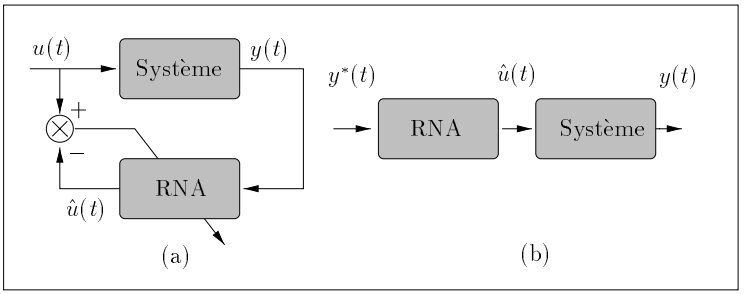
\includegraphics[scale=0.5]{../figures/app2phases.jpg}
 \caption{Apprentissage en deux phases. \textbf{Source}: Gauthier\cite{Gauthier}}
 \label{app2phases}
\end{figure}

Tout d'abord, (a) en boucle, on génère une commande $u$ et on les applique dans le système (\textbf{Figure \ref{app2phases}}).
Soit $y$ l'état du robot après avoir appliqué la commande $u$, on obtient une paire entrée/sortie où $y$ est l'entrée et $u$ la cible.
On continue la boucle pour balayer toutes les configurations possibles de $u$.

Puis vient la phase d'utilisation (b) où on utilise le réseau cette fois pour génèrer les commandes. Mais sans apprentissage. L'adaptabilité est donc sacrifiée.\\

Cette méthode est inadapté au cas où il existe plusieurs commandes idéales pour un même état cible.
En effet, imaginons qu'il éxiste deux commandes idéales pour atteindre le même état cible et que ces deux commandes sont rencontrées lors de la phase (a).
Alors les poids seront modifiés pour converger la sortie vers la première commande idéale rencontrée, puis l'autre et ainsi de suite et finallement, la sortie du réseau pour cet état cible ne va pas converger vers une des commandes idéales.

\subsection{Apprentissage indirecte}
\begin{figure}
 \centering
 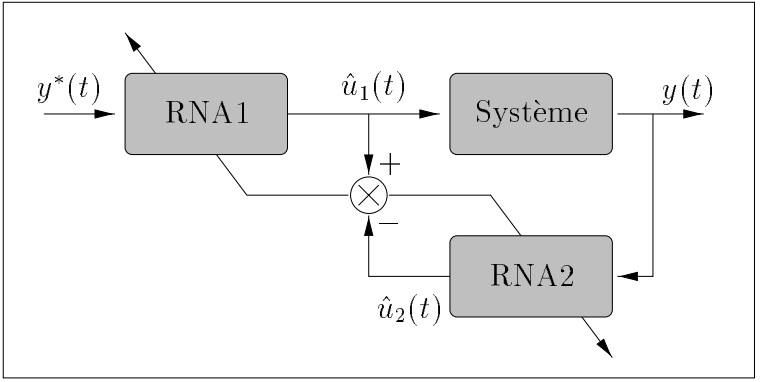
\includegraphics[scale=0.5]{../figures/appindirect.jpg}
 \caption{Apprentissage indirect. \textbf{Source}: Gauthier\cite{Gauthier}}
 \label{appindirect}
\end{figure}

Une méthode qui permet de retrouver l'adaptabilité qui est sacrifiée dans l'apprentissage en deux phases, section \ref{app2phases} (\textbf{Figure \ref{appindirect}}).
RNA1 et RNA2 ne sont pas deux réseaux différents. Il s'agit du même réseau de neurones et RNA1 et RNA2 partagent les mêmes poids.
Mais selon Gauthier\cite{Gauthier}, cette méthode tend à toujours donner la même commande.

\subsection{Apprentissage par modèle différentiable}\label{sec:appmodele}
\begin{figure}
 \centering
 
\includegraphics[scale=0.5]{../figures/invalid.png}
 \caption{Apprentissage par modèle différentiable. \textbf{Source}: Gauthier\cite{Gauthier}}
 \label{appmodele}
\end{figure}

L'idée ici est d'utiliser la méthode de l'apprentissage spécialisé à la section \ref{sec:appspecial} mais en se servant d'un \rna comme modèle différentiable (\textbf{Figure \ref{appindirect}}).
Il faut donc dans un premier temps établir un \rna qui va apprendre à prédire l'état du robot selon la commande à éxecuter.
Nous n'avons pas le problème de l'apprentissage avec maître distant pour ce \rna.
Ensuite, on l'utilise comme modèle. Et là nous pouvons connaître $\partiel{\varepsilon_y}{\hat{u}_1}$ grâce aux formule de rétropropagation de la section \ref{sec:appmlp}.\\
%TODO prouver et parler aussi de formule de backpropagation pour rbf

L'adaptabilité est sacrifiée ici car si le système change et que le modèle n'a pas été entrainé pour ce nouveau système, l'algorithme de rétropropagation va converger la solution vers des commandes inadaptés pour le nouveau système.

\subsection{Apprentissage sur plusieurs étapes}
Un autre problème qui peut se présenter pour la commande par réseaux de neurones est d'obtenir un maître distant seulement après plusieurs étapes.
Par exemple, imaginons que nous voulons commander la marche d'un robot avec un réseau de neurones qui fournira des commandes tous les $T$ secondes.
Si le robot tombe et que nous pouvons en obtenir un maître, nous ne savons pas à quelles étapes avant la chutte le réseau a fourni des commandes responsables de la chutte.\\

Une solution à ce problème est l'architecture de Nguyen et Widrow, Figure \ref{appNguyenWidrow}.
\begin{figure}
 \centering
 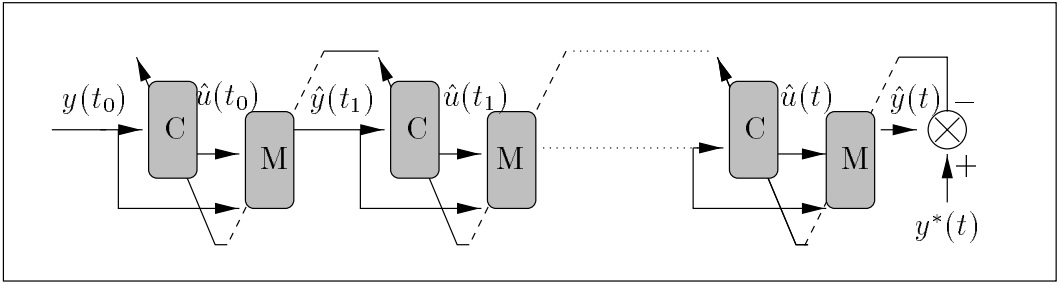
\includegraphics[scale=0.5]{../figures/appNguyenWidrow.jpg}
 \begin{itemize}
  \item \textbf{C}: Réseau qui génère les commandes
  \item \textbf{M}: Modèle
 \end{itemize}
 \caption{Architecture de Nguyen et Widrow. \textbf{Source}: Gauthier\cite{Gauthier}}
 \label{appNguyenWidrow}
\end{figure}
Cela consiste à utiliser un modèle différentiable, qui peut-être un réseau de neurone, pour pouvoir effectuer l'algorithme de rétropropagation jusque la première étape après l'obtention du maître précédent.